
\section{Architecture du FLIR et hypothèses de modélisation}\label{partie2}

\begin{obj}
Vérifier que le choix de l'architecture du FLIR permet de satisfaire les performances établies en partie \ref{partie1}.
Valider des hypothèses simplificatrices afin de pouvoir évaluer les performances du FLIR.
\end{obj}

\subsection{Description et validation de l'architecture du FLIR}

\begin{obj}
Valider le choix de l'architecture du FLIR.
\end{obj}

Le FLIR, fixé au porteur, est constitué :
\begin{itemize}
\item d'un axe motorisé d'\textit{azimut} orientable en rotation par rapport au porteur autour de l'axe $\axe{P}{{z_p}}$ ;
\item d'un ensemble de caméras, appelé \textit{charge}, encastré sur un \textit{axe motorisé d'élévation} orientable en rotation
par rapport à l'axe motorisé d'azimut autour de l'axe $\axe{P}{{y_e}}$.
\end{itemize}

Le modèle cinématique du FLIR et son paramétrage sont donnés sur la figure \ref{figure7}.

\begin{figure}[!htb]
\begin{center}
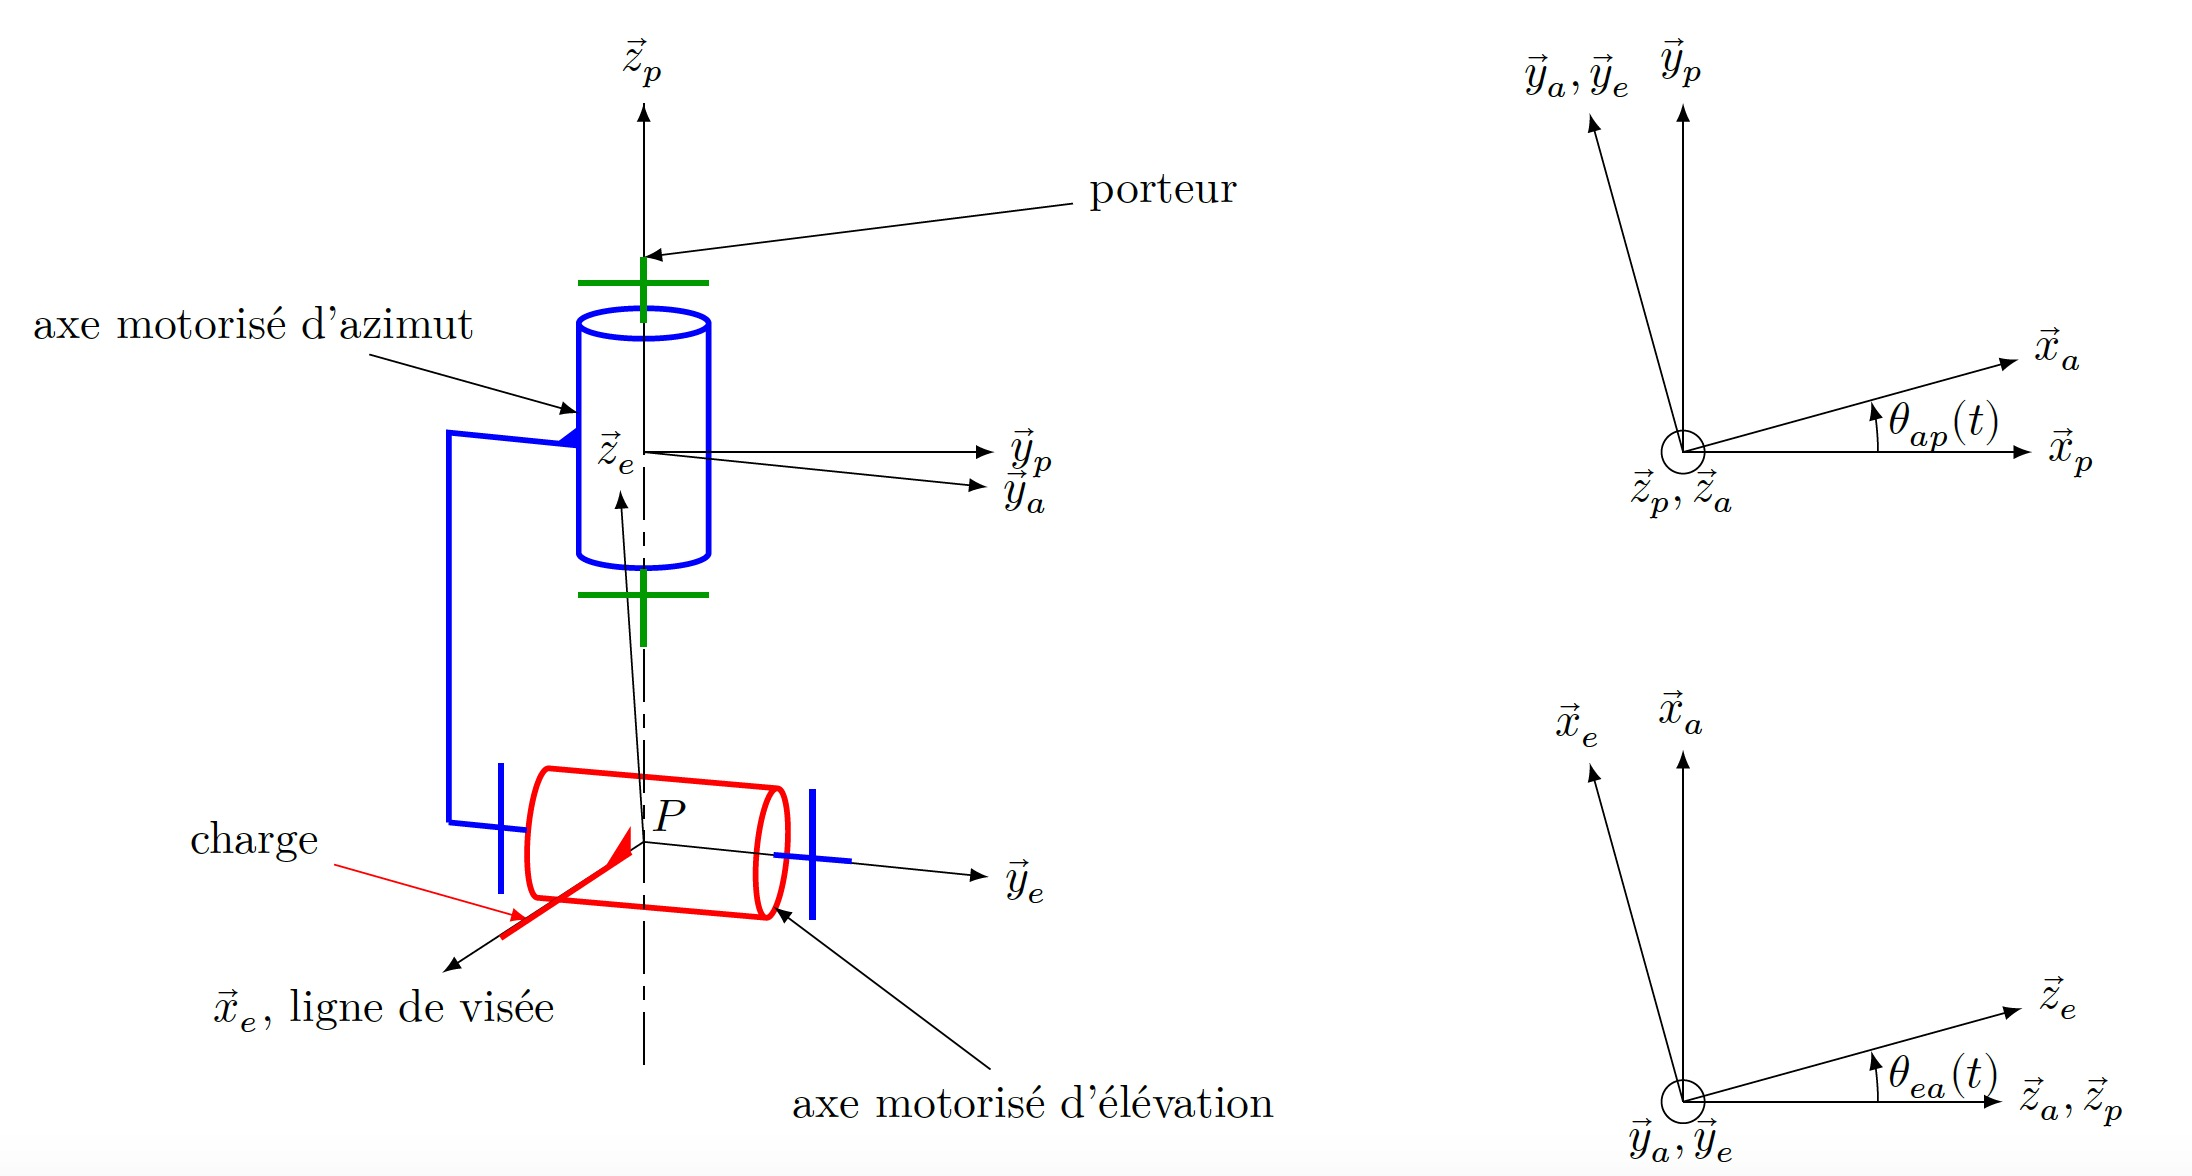
\includegraphics[width=0.9\textwidth]{figure7.jpg}
\caption{Modèle cinématique global paramétré du FLIR, motorisations enlevées \label{figure7}}
\end{center}
\end{figure}

Les repères associés aux solides sont les suivants :
\begin{itemize}
\item $R_a\quadruplet{P}{\vect{x_a}}{\vect{y_a}}{\vect{z_a}}$ pour l'axe motorisé d'azimut ;
\item $R_e\quadruplet{P}{\vect{x_e}}{\vect{y_e}}{\vect{z_e}}$ pour l'ensemble $\left\{\text{axe motorisé d'élévation, charge}\right\}$ dont la ligne de visée est portée par $\vect{x}_e$ ;
\item $R_p\quadruplet{P}{\vect{x_p}}{\vect{y_p}}{\vect{z_p}}$ pour le porteur ;
\item $R_0\quadruplet{P}{\vect{x_0}}{\vect{y_0}}{\vect{z_0}}$ référentiel terrestre non géocentrique, placé à la surface de la Terre au voisinage du porteur avec $\vect{z}_0$ vertical ascendant.
\end{itemize}

Dans la suite du sujet, le référentiel \textbf{$R_0$} est considéré comme galiléen.

\begin{figure}[!htb]
\begin{center}
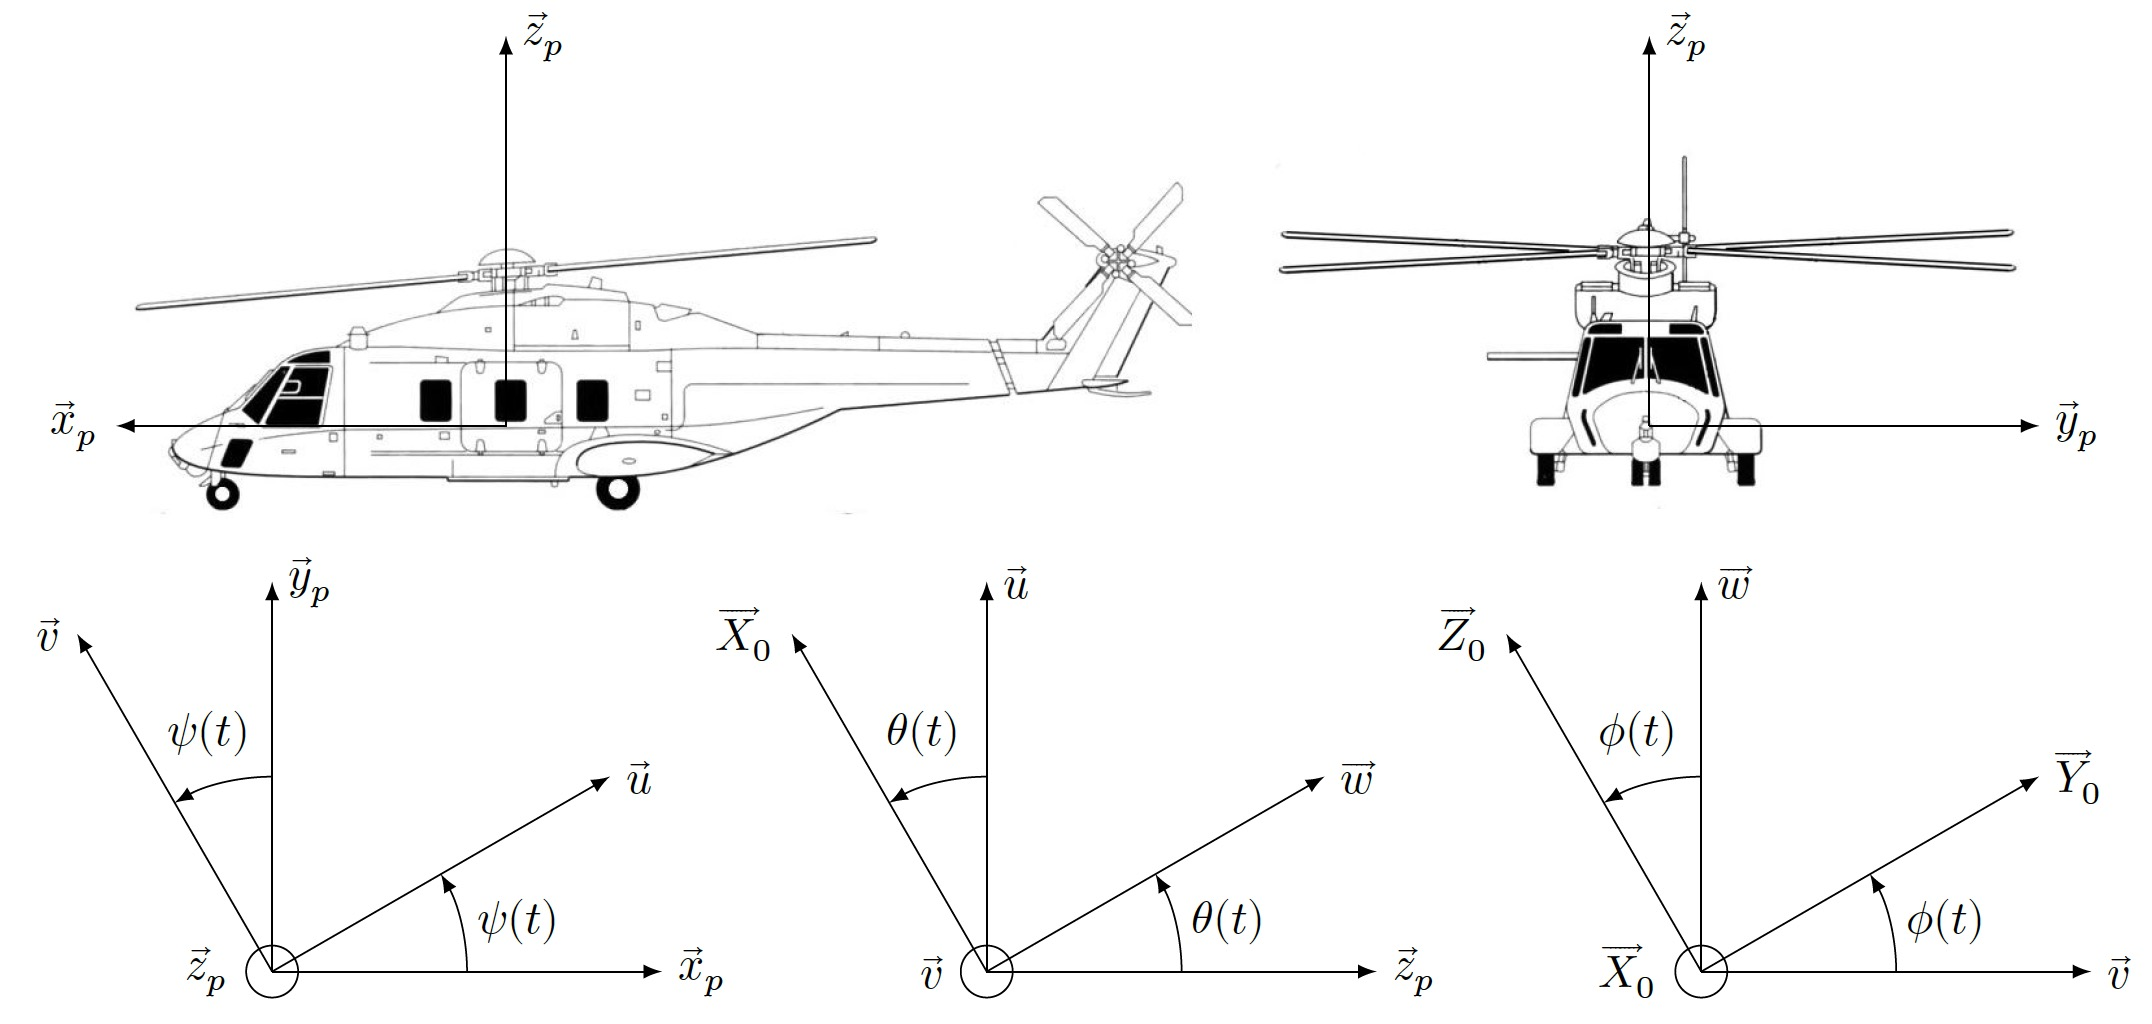
\includegraphics[width=0.9\textwidth]{figure8.jpg}
\caption{Porteur NH90 et son orientation par rapport au référentiel terrestre \label{figure8}}
\end{center}
\end{figure}

Le passage du référentiel terrestre $R_0$ au repère du porteur $R_p$ se fait par l'intermédiaire des trois angles de
Cardan définis sur la figure \ref{figure8}, avec :
\begin{itemize}
\item $\phi(t)$ l'angle de roulis ;
\item $\theta(t)$ l'angle de tangage ;
\item $\psi(t)$ l'angle de lacet.
\end{itemize}

\question{Déterminer le torseur cinématique en $P$ , exprimé dans la base $\base{{x_a}}{{y_a}}{{z_a}}$ de la liaison équivalente
entre le porteur et la charge. En déduire la nature de cette liaison équivalente et préciser ses caractéristiques
géométriques.}

Dans un cas d'utilisation normal, la liaison cinématique entre la tête du pilote et le cockpit est assimilable à une
liaison sphérique dont le centre se trouve au milieu de la nuque. Or, le pilote doit avoir une image cohérente à
sa vision quelle que soit l'orientation de sa tête par rapport au porteur.

\question{Afin de pouvoir valider la solution technique retenue pour la structure cinématique à deux axes orthogonaux
motorisés du FLIR, comparer les mobilités du FLIR et celles de la tête du pilote par rapport au porteur
et expliquer quel doit être un des rôles de l'algorithme implanté dans le calculateur.}

\section{Hypothèses simplificatrices}

\begin{obj}
Valider les hypothèses simplificatrices suivantes :
\begin{itemize}
\item la commande de l'axe motorisé d'azimut est indépendante des mouvements de l'axe motorisé
d'élévation ;
\item  les effets aérodynamiques et la variation de position du centre d'inertie de la charge n'influent pas
sur les performances du FLIR.
\end{itemize}

\end{obj}



%%%%% POUR DM %%%%%

%\subsection{Limitation de l'étude à l'axe motorisé d'élévation}
%La charge mue par l'axe motorisé d'élévation est essentiellement constituée de caméras et de cartes électroniques
%associées. Les ingénieurs ont choisi de disposer ces composants de telle sorte que la répartition des masses de
%cette charge s'approche au mieux de celle d'un cylindre plein et homogène d'axe $\axe{P}{{y_e}}$ de la figure \ref{figure7}.
%
%\question{Justifier que le choix de la répartition des composants de la charge, dans le cas du mouvement simultané
%des deux axes motorisés décrits sur la figure \ref{figure7}, permet de commander l'axe d'azimut indépendamment de l'axe
%motorisé d'élévation.}
%
%Les résultats d'essais en vol montrent que l'axe qui subit le plus de perturbations est l'axe motorisé d'élévation.
%Les commandes des axes d'élévation et d'azimut étant indépendantes l'une de l'autre, la suite de l'étude se
%limitera uniquement à l'axe motorisé d'élévation.

%%%%

\subsection{Rigidité de la structure à double étage de l'axe motorisé d'élévation et influence des
perturbations aérodynamiques}


Afin de limiter l'influence des vibrations du porteur sur la
ligne de visée et augmenter la précision de son orientation,
les ingénieurs ont choisi de décomposer l'axe motorisé
d'élévation en deux étages (voir figures \ref{fig9} et \ref{figure10}).
Le premier étage, appelé étage gros d'élévation ($ge$), est
en prise directe avec l'air et est donc soumis aux effets
aérodynamiques lors des mouvements du porteur. L'étage
gros d'élévation est lui même en liaison pivot, d'axe $\axe{P}{{y_e}}$,
avec l'axe motorisé d'azimut.

\begin{figure}[h]
\begin{center}
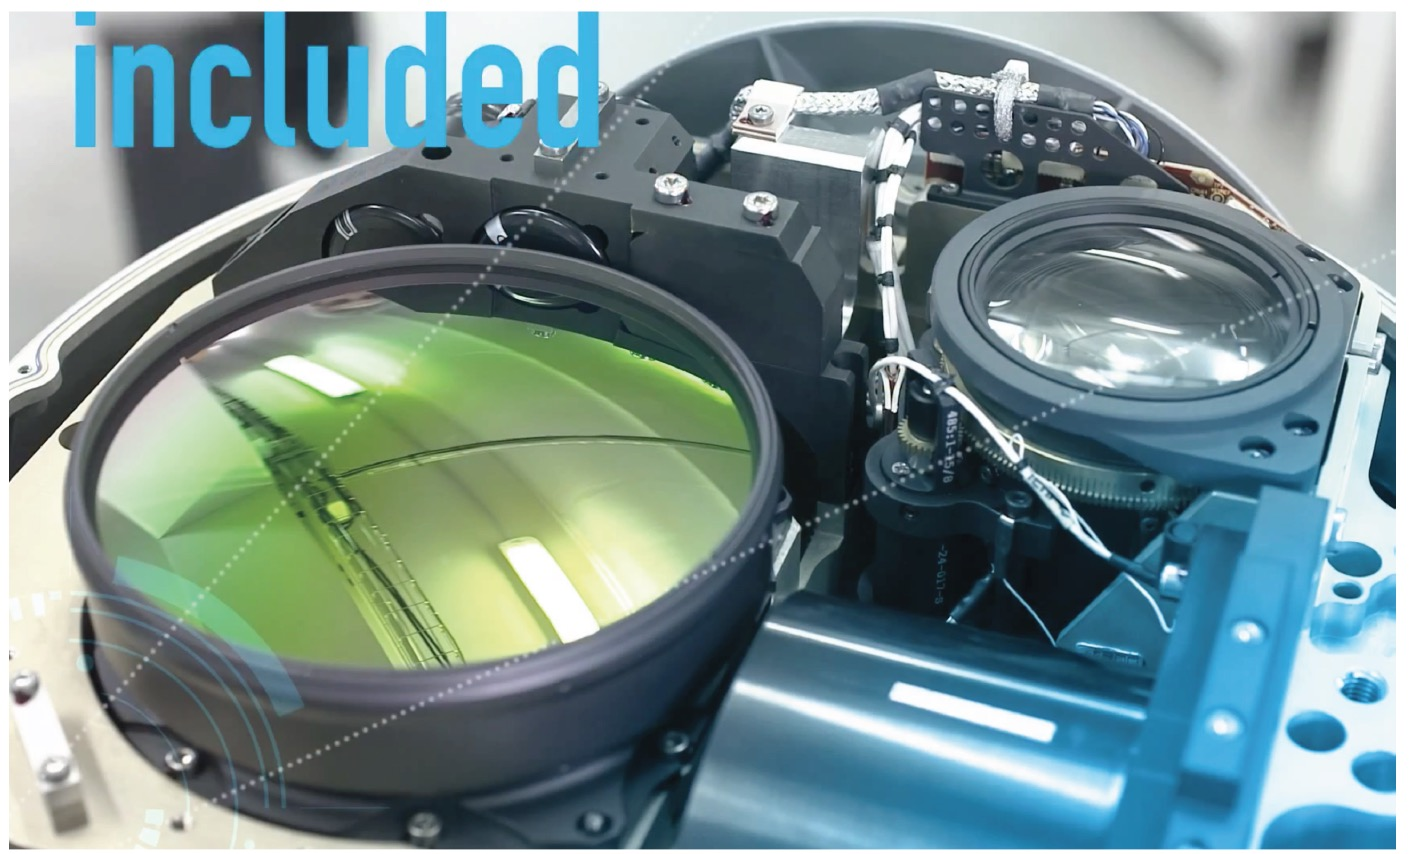
\includegraphics[width=0.4\textwidth]{figure9.jpg}
\caption{Intérieur du FLIR, vue des optiques des caméras liées à l'étage fin d'élévation\label{fig9}}
\end{center}
\end{figure}

%\FloatBarrier

Le second, appelé étage fin d'élévation ($fe$), est protégé
des effets aérodynamiques grâce au carter sphérique
solidaire de l'étage gros. Cet étage est en liaison pivot,
d'axe $\axe{P}{{y_e}}$, avec l'étage gros d'élévation. L'inertie des
éléments déplacés par l'étage fin d'élévation est plus faible
que celle de l'étage gros d'élévation et les choix de guidage
et de motorisation permettent d'atteindre des accélérations
et des vitesses élevées. Cependant, l'amplitude du mouvement de l'étage fin est limitée.

\begin{figure}[!htb]
\begin{center}
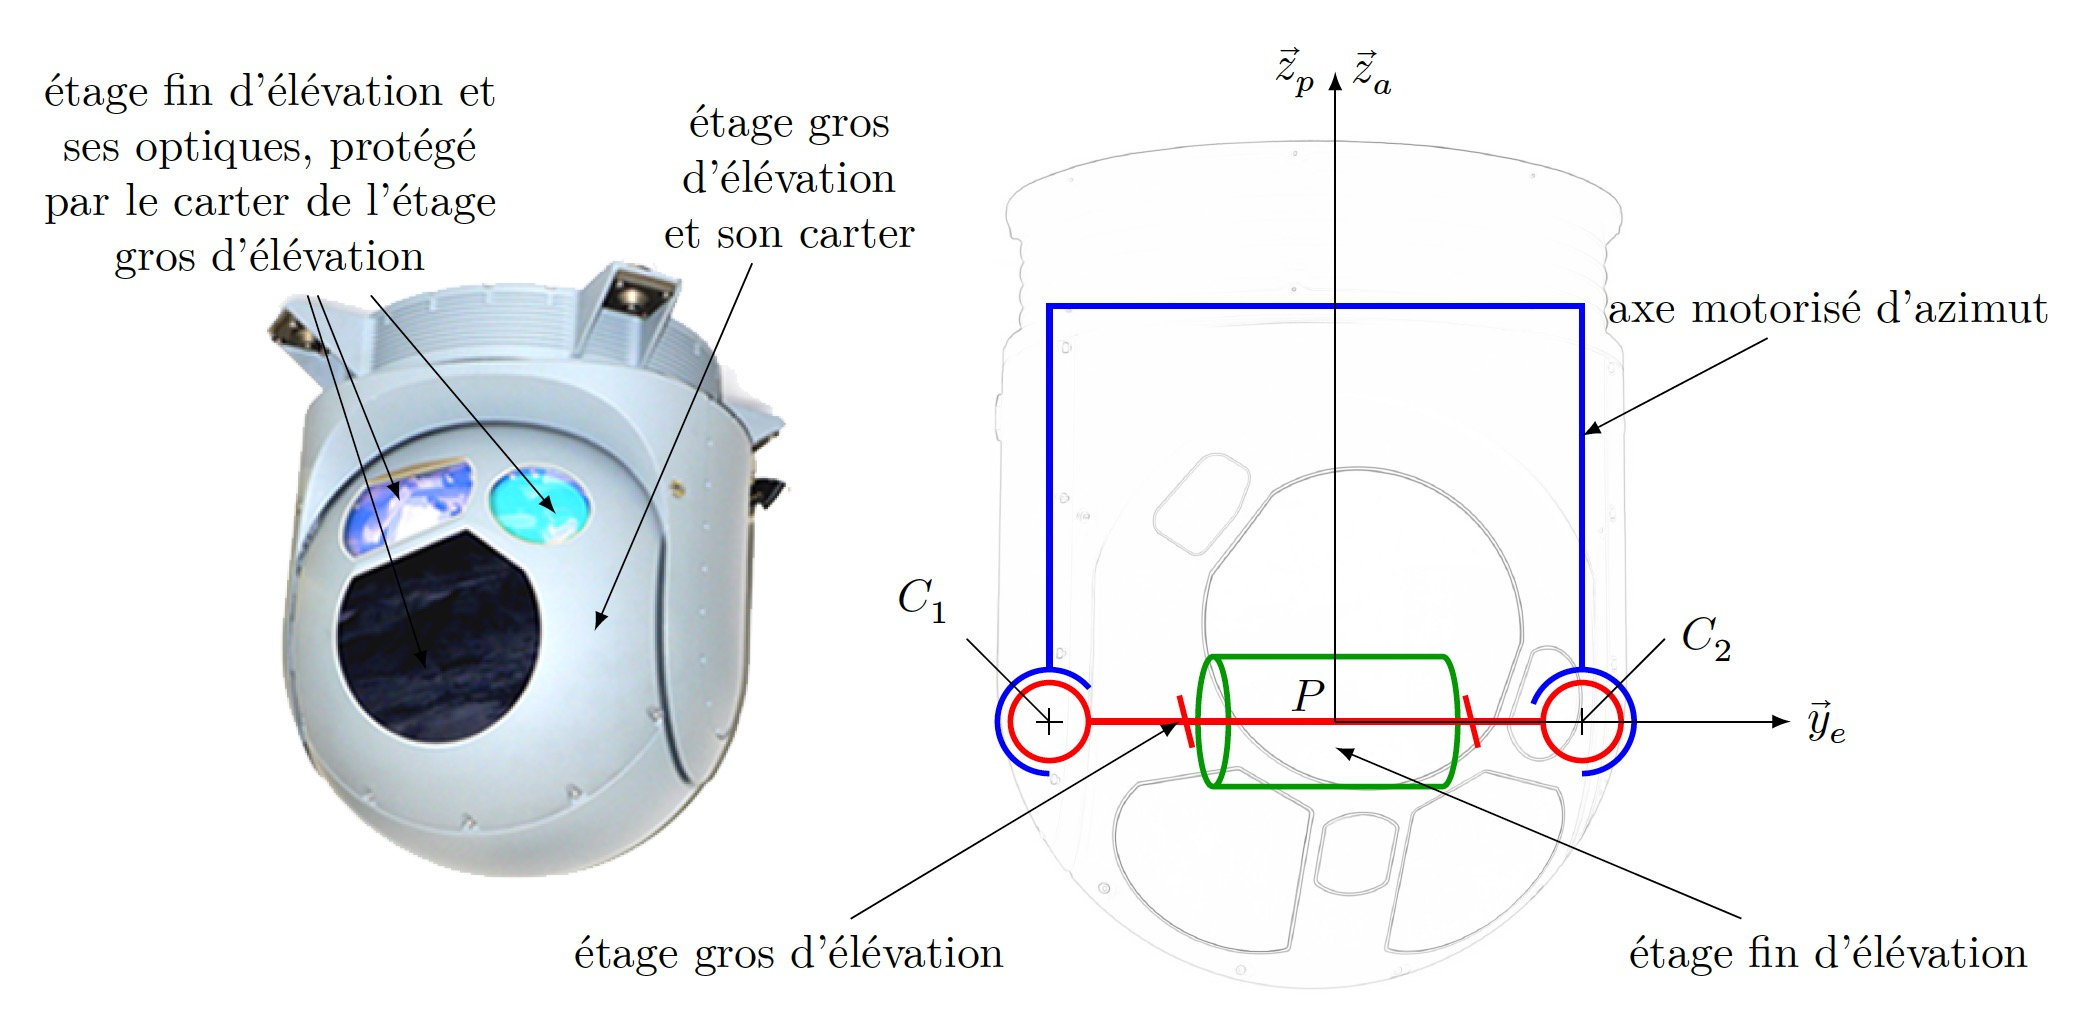
\includegraphics[width=0.9\textwidth]{figure10.jpg}
\caption{FLIR et modèle cinématique de l'axe motorisé d'élévation \label{figure10}}
\end{center}
\end{figure}

Le guidage en rotation entre l'étage gros d'élévation et l'axe motorisé d'azimut est réalisé à l'aide de deux
composants à éléments roulants modélisables par des liaisons sphériques de centre $C_1$ et $C_2$.

\question{À l'aide de la figure \ref{figure10}, déterminer le degré
d'hyperstatisme du modèle du guidage en rotation
entre l'axe motorisé d'azimut et l'étage gros d'élévation.
Lister deux avantages et un inconvénient
de ce guidage, puis conclure quant à sa pertinence
vis-à-vis de la précision de l'orientation de la ligne
de visée souhaitée.}

Le montage de l'étage gros d'élévation sur l'axe motorisé
d'azimut induit des efforts axiaux égaux, opposés
et dirigés suivant $\vect{y}_e$, dans les liaisons de centre
$C_1$ et $C_2$. Ces efforts, appelés précharge, sont réglables
au montage en jouant sur la différence de distance
entre les points $C_1$ et $C_2$ prise d'une part, sur
l'axe motorisé d'azimut et, d'autre part, sur l'étage
gros d'élévation.


\begin{figure}[h]
\begin{center}
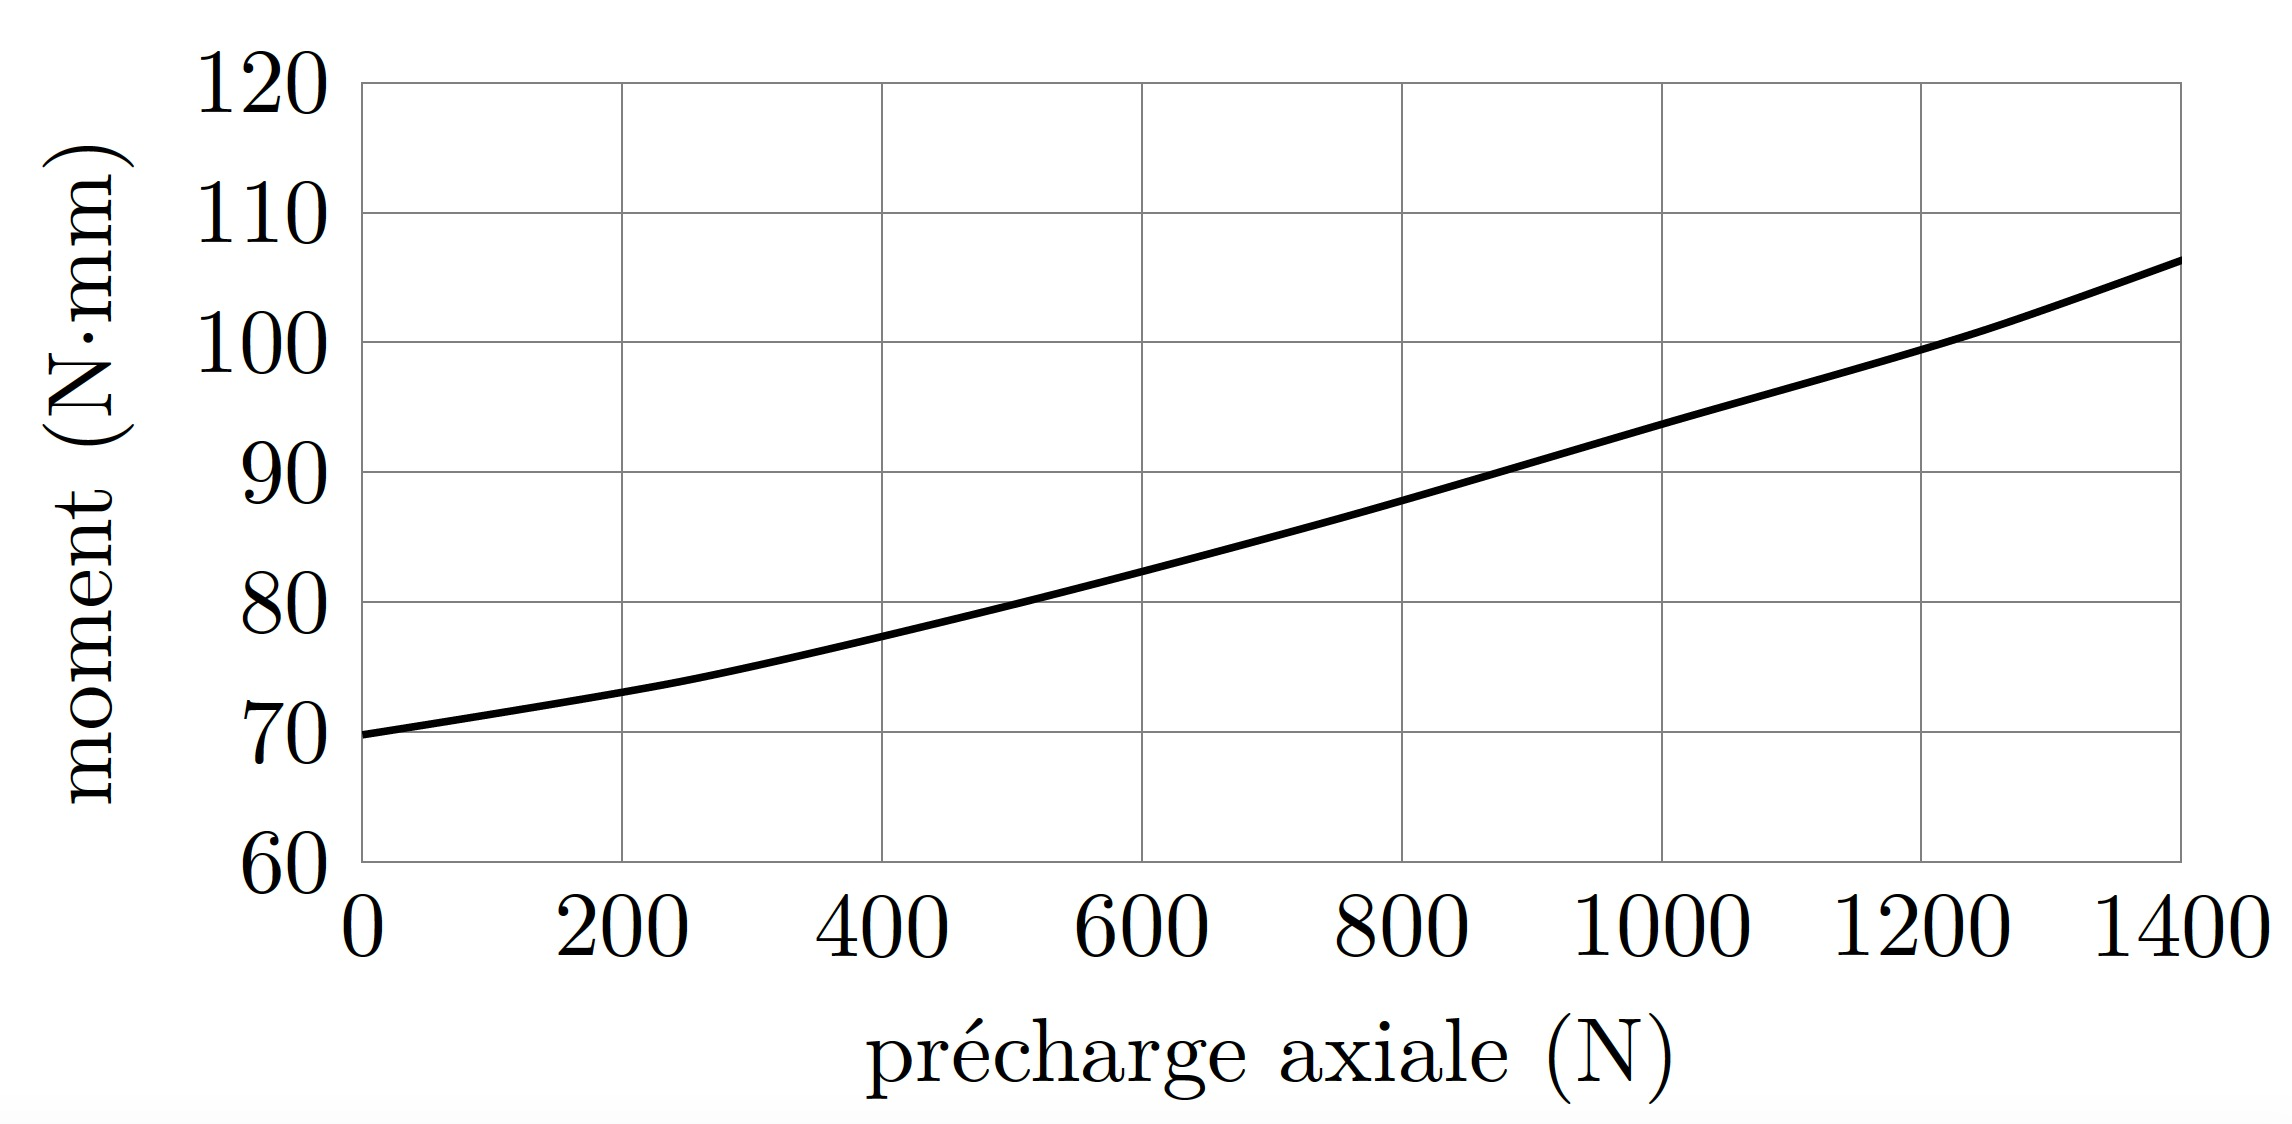
\includegraphics[width=0.5\textwidth]{figure11.jpg}
\caption{Moment de frottement sec d'un seul composant à éléments roulants du guidage en rotation de l'étage
gros d'élévation par rapport à l'axe motorisé d'azimut, en fonction de la précharge axiale (source : SKF)\label{fig11}}
\end{center}
\end{figure}
%\FloatBarrier

Lors des conditions de vol les plus sévères, le couple exercé par les effets aérodynamiques sur le carter de l'étage
gros d'élévation a été mesuré à $\SI{0,18}{N.m}$.

\question{À l'aide de l'abaque donné figure \ref{fig11}, déterminer une valeur de réglage pertinente de la précharge du guidage en rotation de l'étage gros d'élévation par rapport à l'axe motorisé d'azimut.}

%\FloatBarrier
\subsection{Influence du déport de masse lié à la variation de position des optiques}

Le déplacement des optiques (zoom) en translation rectiligne suivant $\vect{x}_e$ par rapport à l'étage fin d'élévation
rend la géométrie de ce dernier variable et son centre d'inertie ne se situe pas exactement sur l'axe de rotation
$\axe{P}{{y_e}}$ de l'étage fin d'élévation par rapport à l'étage gros d'élévation.
L'étage fin d'élévation est modélisé par l'ensemble des deux solides suivants (voir figure \ref{figure12}) :
\begin{itemize}
\item un disque plein et homogène d'axe $\axe{P_0}{{x_e}}$ de masse $m_o$, de rayon $r_o$ et de centre de gravité $P_o$, modélisant les optiques mobiles de l'étage fin d'élévation ;
\item un cylindre plein et homogène d'axe $\axe{P}{{y_e}}$ de masse $\indice{m}{cyl}$, de rayon $\indice{r}{cyl}$, de hauteur $\indice{h}{cyl}$ et de centre de gravité $P$, modélisant le reste des éléments de l'étage fin d'élévation.
\end{itemize}

Dans la suite, ces deux solides sont supposés être en liaison complète, c'est-à-dire que la distance $d$, telle que $\vect{PP_0}=d\vect{x_e}$ est constante.

\begin{figure}[!htb]
\begin{center}
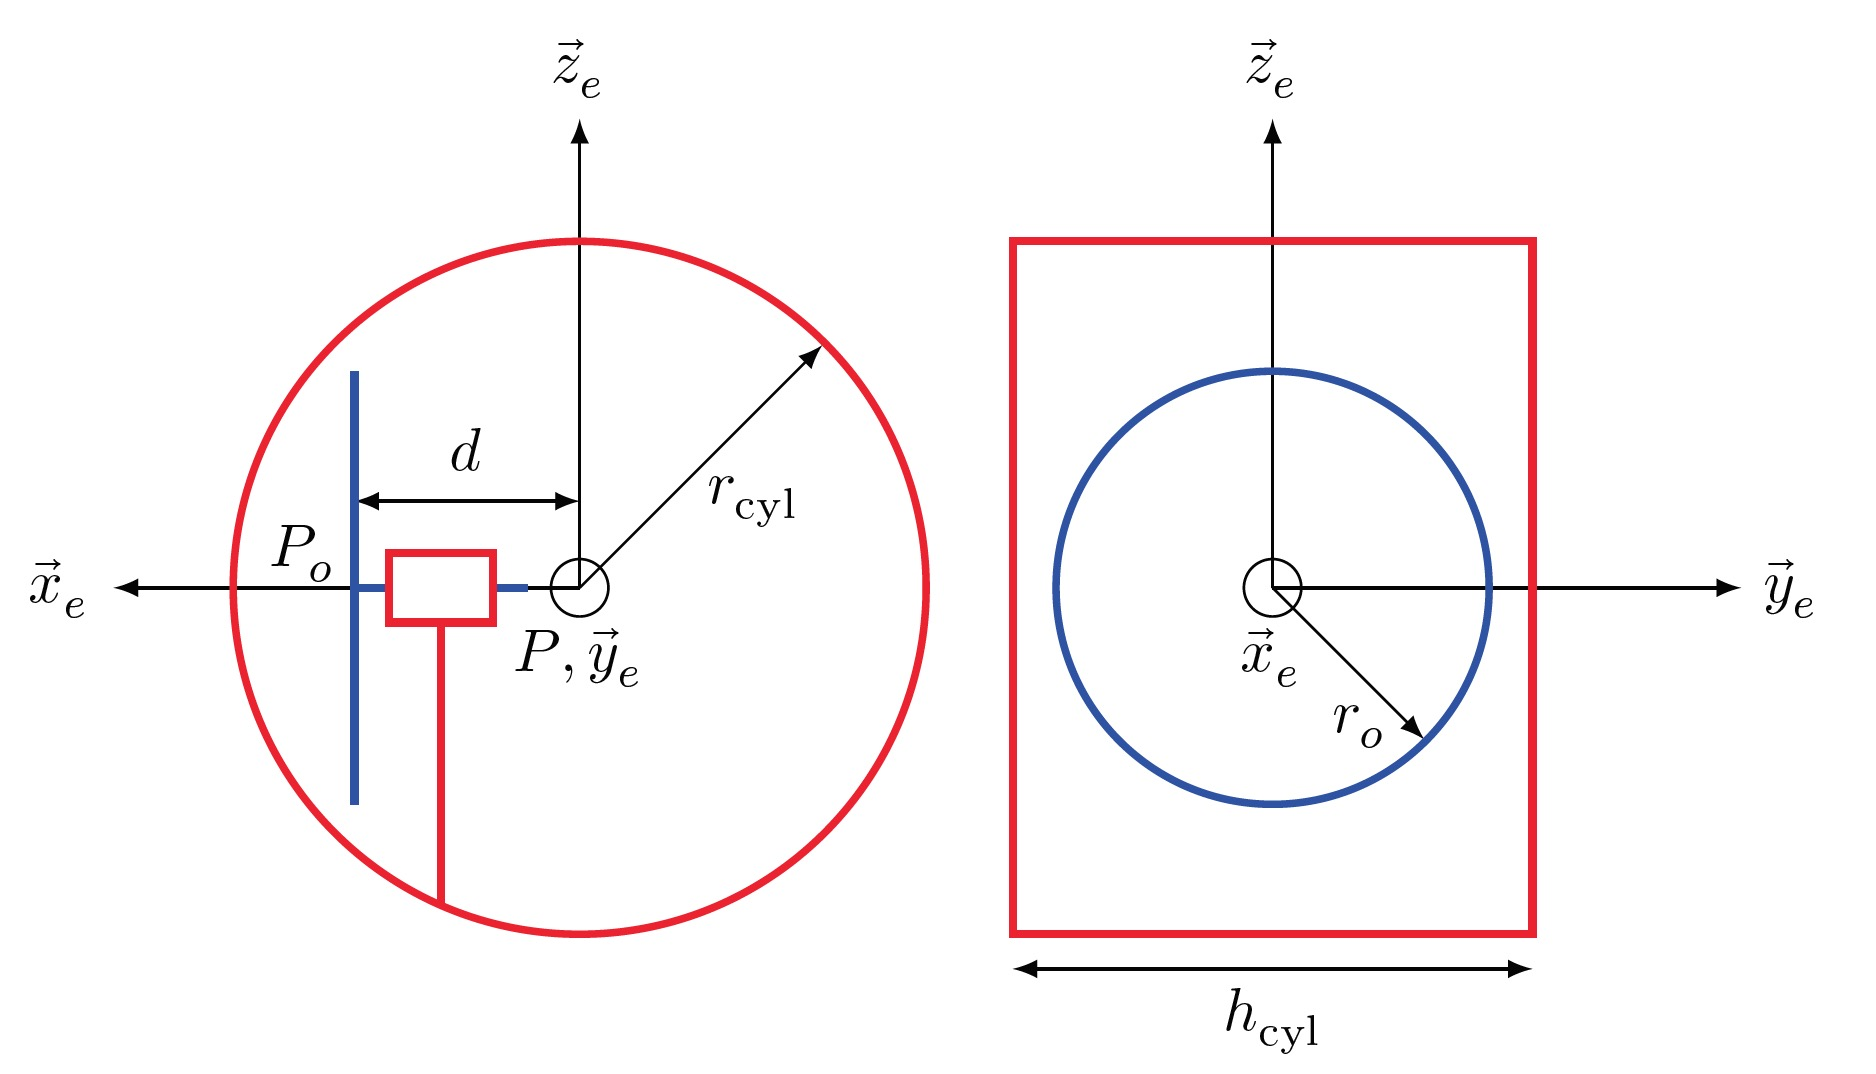
\includegraphics[width=0.6\textwidth]{figure12.jpg}
\caption{Modélisation de la géométrie des masses de l'étage fin d'élévation \label{figure12}}
\end{center}
\end{figure}

\begin{itemize}
\item L'opérateur d'inertie du cylindre plein, noté $cyl$, est de la forme suivante :
$
\overline{\overline{I}}_P(\text{cyl})=
\left(
\begin{array}{ccc}
\indice{A}{cyl} & 0 & 0 \\ 
0 & \indice{B}{cyl} & 0 \\ 
0 & 0 & \indice{A}{cyl}
\end{array}
\right)_{\base{\vect{x_e}}{\vect{y_e}}{\vect{z_e}}} 
$
\item L'opérateur d'inertie des optiques, noté $o$, est de la forme suivante :
$
\overline{\overline{I}}_{P_o}(o)=
\left(
\begin{array}{ccc}
A_{o} & 0 & 0 \\ 
0 & B_{o} & 0 \\ 
0 & 0 & B_{o}
\end{array}
\right)_{\base{\vect{x_e}}{\vect{y_e}}{\vect{z_e}}} 
$
\item L'étage fin d'élévation est noté $f_e$, sa masse est égale à $\indice{m}{fe}=\indice{m}{cyl}+m_o$, son centre d'inertie est noté $G_{fe}$.
\end{itemize}

\question{Déterminer littéralement l'opérateur d'inertie $\overline{\overline{I}}_P(\text{fe})$ de l'étage fin d'élévation en fonction de $\indice{A}{cyl}$, $\indice{B}{cyl}$, $A_o$, $B_o$, $d$ et $m_o$ dans le repère $R_e$, puis exprimer le vecteur $\vect{PG_{fe}}=\lambda \cdot \vect{x}_e$ dans le repère $R_e$ en fonction de $\indice{m}{cyl}$, $m_o$ et $d$.}

Des mesures à bord du NH90 ont montré que la phase de vol la plus pénalisante, c'est-à-dire celle qui perturbe
le plus la ligne de visée du FLIR, est l'ascension verticale du porteur. Dans cette phase, il est possible d'effectuer
les hypothèses suivantes :
\begin{itemize}
\item les angles $\psi(t)$, $\theta(t)$ et $\phi(t)$ sont constants et nuls ;
\item $\theta_{ap}(t)=0$ ;
\item $\vect{z}_p=\vect{z}_a=\vect{z}_0$ vertical ascendant, $\vect{y}_p=\vect{y}_a=\vect{y}_0$ et $\vect{x}_p=\vect{x}_a=\vect{x}_0$;
\item l'étage fin d'élévation est en mouvement par rapport à l'étage gros d'élévation ;
\item la ligne de visée est définie par l'orientation $\theta_{eo}(t)$ de l'étage fin d'élévation par rapport à $R_0$. Dans cette
étude, $\theta_{e0}(t)=\theta_{ea}(t)$;
\item $R_0$ est galiléen ;
\item le couple moteur sur l'étage fin d'élévation est noté $C_m(t)$ ;
\item la liaison pivot entre l'étage fin d'élévation et l'étage gros d'élévation est supposée parfaite.
\end{itemize}

La vitesse d'ascension verticale du porteur est notée $\vect{V}(P\in \text{porteur}/R_0)=v(t)\cdot \vect{z}_0$ et son accélération est notée $\vect{\Gamma}(P\in \text{porteur}/R_0)=\gamma(t)\cdot \vect{z}_0$.

Les dérivées d'un paramètre $x(t)$ par rapport au temps seront notées : $\dot{x}(t)=\dfrac{\dd x(t)}{\dd t}$ et $\ddot{x}(t)=\dfrac{\dd ^2x(t)}{\dd t^2}$. 

\question{Montrer que $\vect{V}(G_{fe}\in fe/R_0)$, vecteur vitesse du point $G_{fe}$, centre d'inertie de l'étage fin d'élévation dans son mouvement par rapport à $R_0$, peut s'écrire sous la forme : $\vect{V}(G_{fe}\in fe/R_0)=a(t)\cdot \vect{z}_0+b(t)\cdot \vect{z}_e$. L'exprimer alors en fonction de $v(t)$, $m_{cyl}$, $m_o$, $d$, $\theta_{eo}(t)$ et $\dot{\theta}_{eo}(t)$.}


\question{Déterminer l'accélération $\vect{\Gamma\left( G_{\text{fe}},fe/R_0 \right)}$}

\question{Isoler $\text{fe}$ et faire les bilan des actions mécaniques en écrivant tous les torseurs en $P$}

\question{Énoncer le théorème du moment dynamique appliqué à $fe$ en $P$ sans développer le calcul.}

\question{Donner la relation liant le moment dynamique en $P$ ($\vect{\delta\left( P,fe/R_0 \right)}$) à celui en $G_{fe}$ ($\vect{\delta\left( G_{\text{fe}},fe/R_0 \right)}$)}

\question{Déterminer le moment cinétique $\vect{\sigma\left( G_{\text{fe}},fe/R_0 \right)}$ puis le moment dynamique au même point : \(\vect{\delta\left( G_{\text{fe}},fe/R_0 \right)}$}

\question{En déduire le moment dynamique : $\vect{\delta\left( P,fe/R_0 \right)}$}

\question{En déduire l'équation différentielle régissant le mouvement de l'étage fin d'élévation par rapport
au référentiel galiléen $R_0$.}

Les valeurs numériques suivantes sont données : $m_o =\SI{1,4}{kg}$ ; $d= \SI{0,01}{m}$ ; $\vert \gamma(t)\vert_{\text{MAXI NH90}} = \SI{1,8}{g}$, avec $g\approx  \SI{9,81}{m.s^{-2}}$.

Les couples perturbateurs voisins du dixième de la valeur du couple moteur maximal seront négligés vis-à-vis
de ce dernier lors de la conception de la commande. Pour l'étage fin d'élévation, le couple moteur maximal est
voisin de $\SI{3}{N.m}$.

\question{Dans la phase de vol étudiée, donner sous forme littérale l'expression du couple de perturbation issu du déport de masse $d$, noté $\indice{C}{pert}$. Calculer la valeur numérique maximale de $\indice{C}{pert}$, notée $C_{\text{pertMAXI}}$, dans le cas le plus défavorable. Conclure sur la pertinence de la prise en compte de cette perturbation pour la conception de
la commande de l'étage fin d'élévation.}
